\section{Εισαγωγή}

\paragraph{} Οι προσομοιώσεις φυσικών φαινομένων στον υπολογιστή χρησιμοποιούνται
εκτεταμένα για την καλύτερη κατανόηση των φαινομένων αυτών. Η δυνατότητα πρόβλεψης και
ανάλυσης που παρέχουν, τόσο σε πραγματικές όσο και υποθετικές περιπτώσεις, τις καθιστούν
ιδιαίτερα ελκυστικές για επιστήμονες σε τεράστιο αριθμό ερευνητικών πεδίων και
εφαρμογών. Στη σύγχρονη εποχη προγράμματα προσομοιώσεων θεωρούνται αναπόσπαστο εργαλείο
κάθε επιστήμονα στη φυσική, αστροφυσική, γεωλογία, κλιματολογία, χημεία, βιολογία,
οικονομία, ψυχολογία, κοινωνικές επιστήμες όπως και μηχανολόγου, ηλεκτρολόγου, πολιτικού
και χημικού μηχανικού. Η προσομοίωση σαν τεχνική υπερπηδά πολλά από τα εμπόδια που
παρουσιάζονται στην επίλυση των αντίστοιχων προβλημάτων με αναλυτικές μεθόδους. Πολύ
σημαντική για την αξιολόγηση και ερμηνεία των αποτελεσμάτων της προσομοίωσης είναι η
επιλογή του μοντέλου για την αναπαράσταση του συστήματος. Τα μοντέλα ειναι μαθηματικές
περιγραφές του συστήματος, σημαντικά χαρακτηριστικά των οποίων είναι οι απλουστεύσεις
(παράγοντες που δεν λαμβάνονται υπόψη), οι προσεγγίσεις (μη ακριβείς περιγραφές παραγόντων
με σφάλματα που μπορεί να οφείλονται σε δειγματοληψία, κλπ) και οι παραδοχές (υιοθέτηση
αρχών που δεν αντιπροσωπεύουν πλήρως την πραγματικότητα) που γίνονται κατά την ανάπτυξή
τους. Τα παραπάνω γίνονται προκειμένου να καταστεί δυνατή στην πράξη η αριθμητική επίλυση
των εξισώσεων που περιγράφουν το αρχικό σύστημα μέσω του μοντέλου.

\subsection{Προσομοιώσεις Τσουνάμι}
\paragraph{} Ένα από τα πιο πρόσφορα και ανεπτυγμένα πεδία εφαρμογών των προσομοιώσεων
ειναι η ρευστοδυναμική, όπου αντίστοιχα εργαλεία χρησιμοποιούνται ευρύτατα από επιστήμονες
και μηχανικούς. Παραδείγματα αποτελούν η μελέτη της ροής του αίματος στα αγγεία, του αέρα
στους πνεύμονες, αεροδυναμικής-υδροδυναμικής κατά το σχεδιασμό οχημάτων, σκαφών και
υδάτινων εγκαταστάσεων (γέφυρες, φράγματα), μετεωρολογία κα. Ιδιαίτερα για την πρόβλεψη,
καταγραφή, προσομοίωση και ανάλυση φυσικών φαινομένων και ειδικά μεγάλης κλίμακας, όπως
τυφώνες, σεισμοί, τσουνάμι, έχουν επενδυθεί τεράστιοι πόροι από πολλές χώρες όπως οι ΗΠΑ,
η Ιαπωνία και η Κίνα. Ειδικά για τα τσουνάμι έχουν δημιουργηθεί πολλά συστήματα
παρακολούθησης και προειδοποίησης τα οποία επεξεργαζόμενα δεδομένα από πλωτές σημαδούρες,
βυθομετρικούς αισθητήρες πίεσης, σεισμογράφους αλλά και τοπογραφικούς χάρτες του
υποθαλάσσιου αναγλύφου επιτυγχάνουν με τη βοήθεια υπολογιστικών μοντέλων έγκαιρη πρόγνωση
σχετικά με τις περιοχές προσβολής και το χρονικό περιθώριο για επικείμενα τσουνάμι. Δύο
από τα μεγαλύτερα τέτοια συστήματα είναι το \eng{PTWC} και το \eng{NTWC} (\eng{Pacific}
και \eng{National Tsunami Warning Center}), τα οποία συστάθηκαν από τη \eng{NOAA}
(\eng{National Oceanic and Atmospheric Administration}), κυβερνητική υπηρεσία των ΗΠΑ. Το
\eng{PTWC} με έδρα στο \eng{'Ewa Beach} της Χαβάης αποτελεί τμήμα διεθνούς συστήματος
πρόγνωσης τσουνάμι, με κύρια περιοχή παρακολούθησης τον Ειρηνικό Ωκεανό. Το \eng{NTWC} στο
\eng{Palmer} της Αλάσκα εξυπηρετεί όλες τις παράκτιες περιοχές του Καναδά και των ΗΠΑ
εκτός της Χαβάης, της Καραϊβικής και του Κόλπου του Μεξικού. Μετά το σεισμό και το
τσουνάμι του 2004 στον Ινδικό Ωκεανό το \eng{PWTC} επέκτεινε τις προειδοποιήσεις για
τσουνάμι και στην περιοχή του Ινδικού Ωκεανού, της Καραϊβικής και των γειτονικών περιοχών,
μέχρι την ανάληψη αυτών από τοπικές υπηρεσίες. Αυτό έχει ήδη συμβεί για τον Ινδικό Ωκεανό,
όπου το έργο αυτό επιτελούν από κοινού η \eng{JATWC} (\eng{Joint Australian Tsunami
  Warning Centre}), η \eng{INCOIS} (\eng{Indian National Centre for Ocean Information
  Services}) και η \eng{BMKG} (\eng{Meteorological, Climatological and Geophysical Agency
  of Indonesia}). Περιοχές με υψηλό κίνδυνο πλήγματος από τσουνάμι διαθέτουν επιπρόσθετα
τοπικά συστήματα συναγερμού και προειδοποιητικές πινακίδες (εικόνα
\ref{fig:tsunami-signs}).

\begin{figure}[h]
  \begin{subfigure}{.5\textwidth}
    \centering
    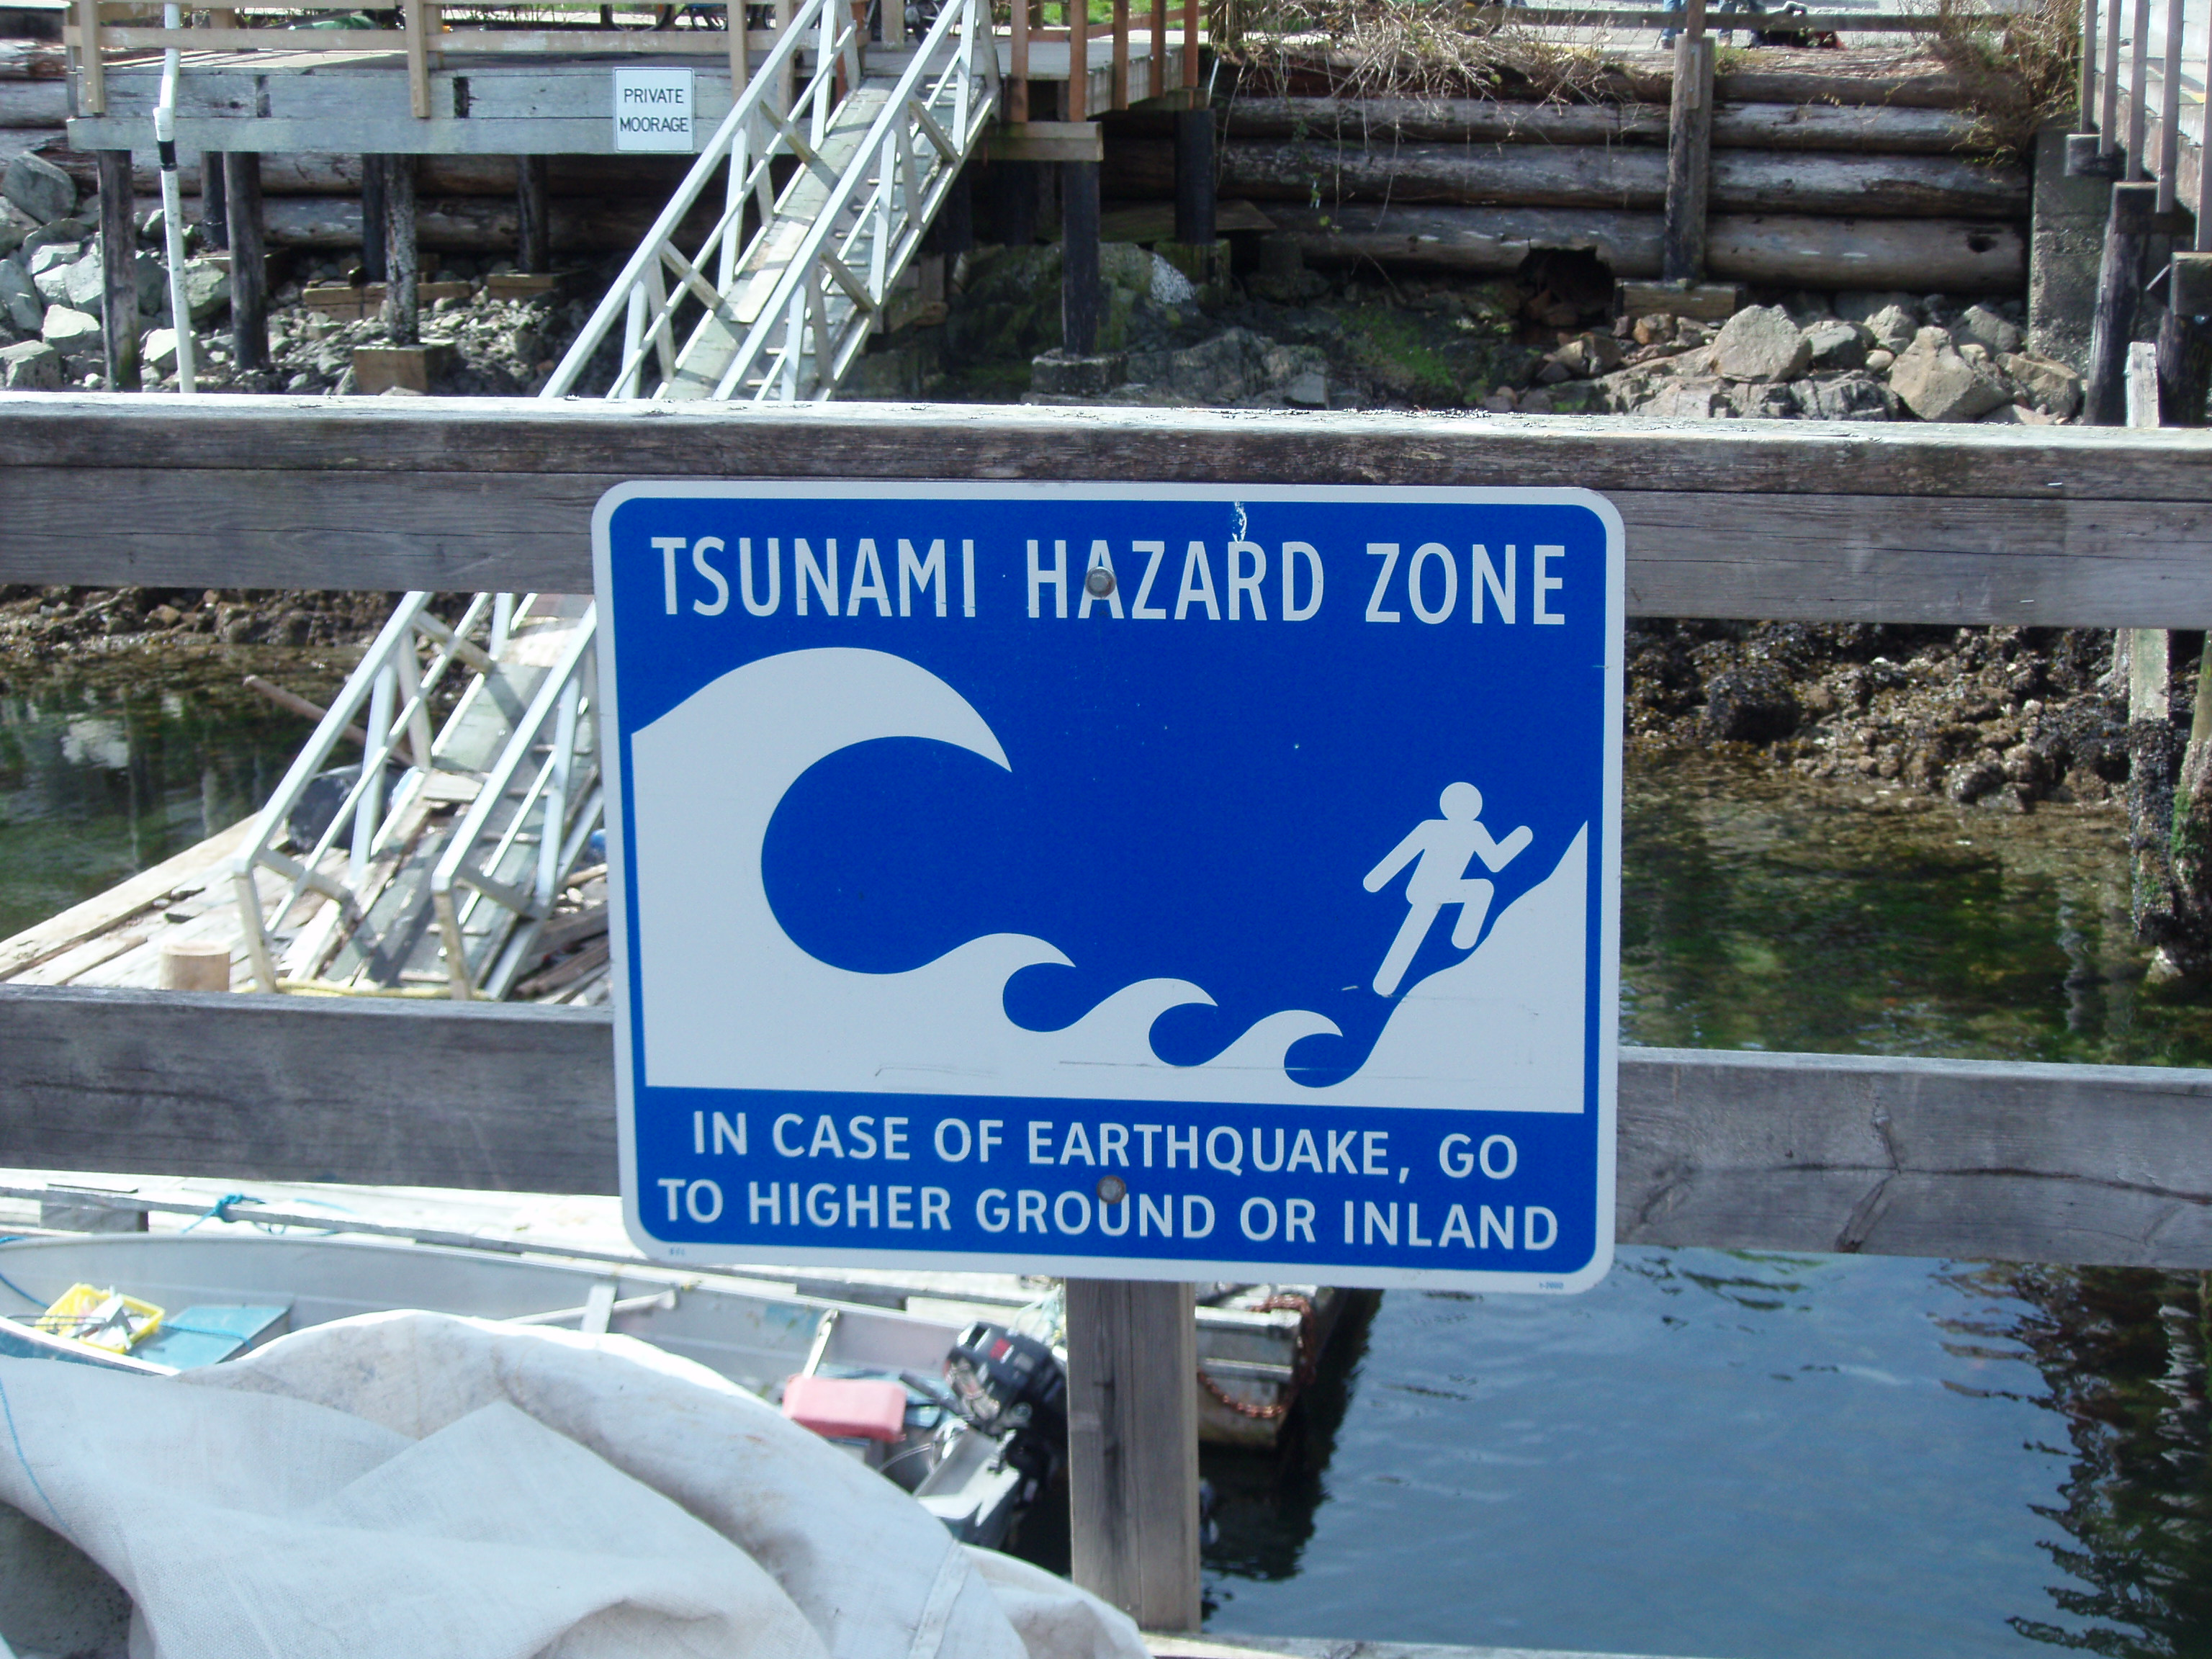
\includegraphics[width=\textwidth]{figures/tsunami-sign-0.jpg}
  \end{subfigure}
  \begin{subfigure}{.5\textwidth}
    \centering
    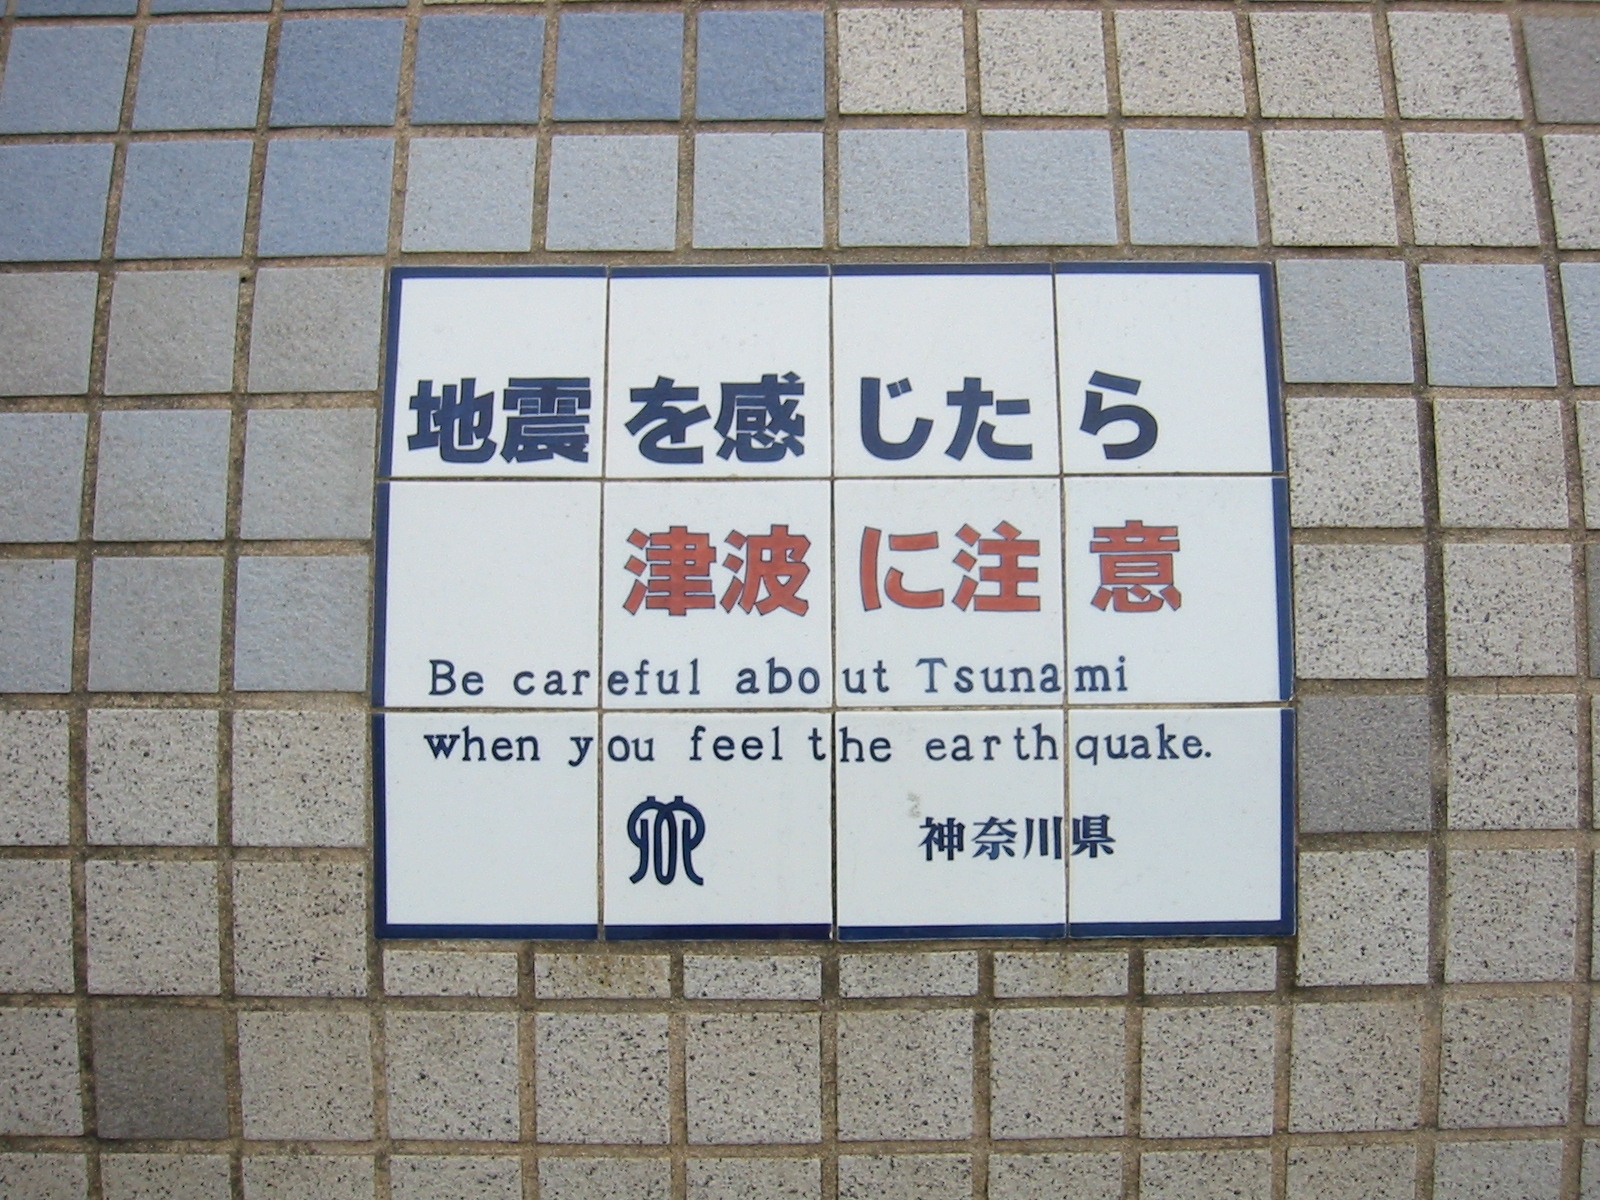
\includegraphics[width=\textwidth]{figures/tsunami-sign-1.jpg}
  \end{subfigure}
  \caption[Προειδοποιητικές πινακίδες σε περιοχές υψηλού κινδύνου]{Πινακίδες που
    προειδοποιούν σε περιοχές με υψηλό κίνδυνο πλήγματος από τσουνάμι. Αριστερά στο
    \eng{Bamfield, British Columbia} στον Καναδά και δεξιά στην πόλη \eng{Kamakura} στην
    Ιαπωνία.}
  \label{fig:tsunami-signs}
\end{figure}

\begin{figure}[h]
  \begin{subfigure}{.5\textwidth}
    \centering
    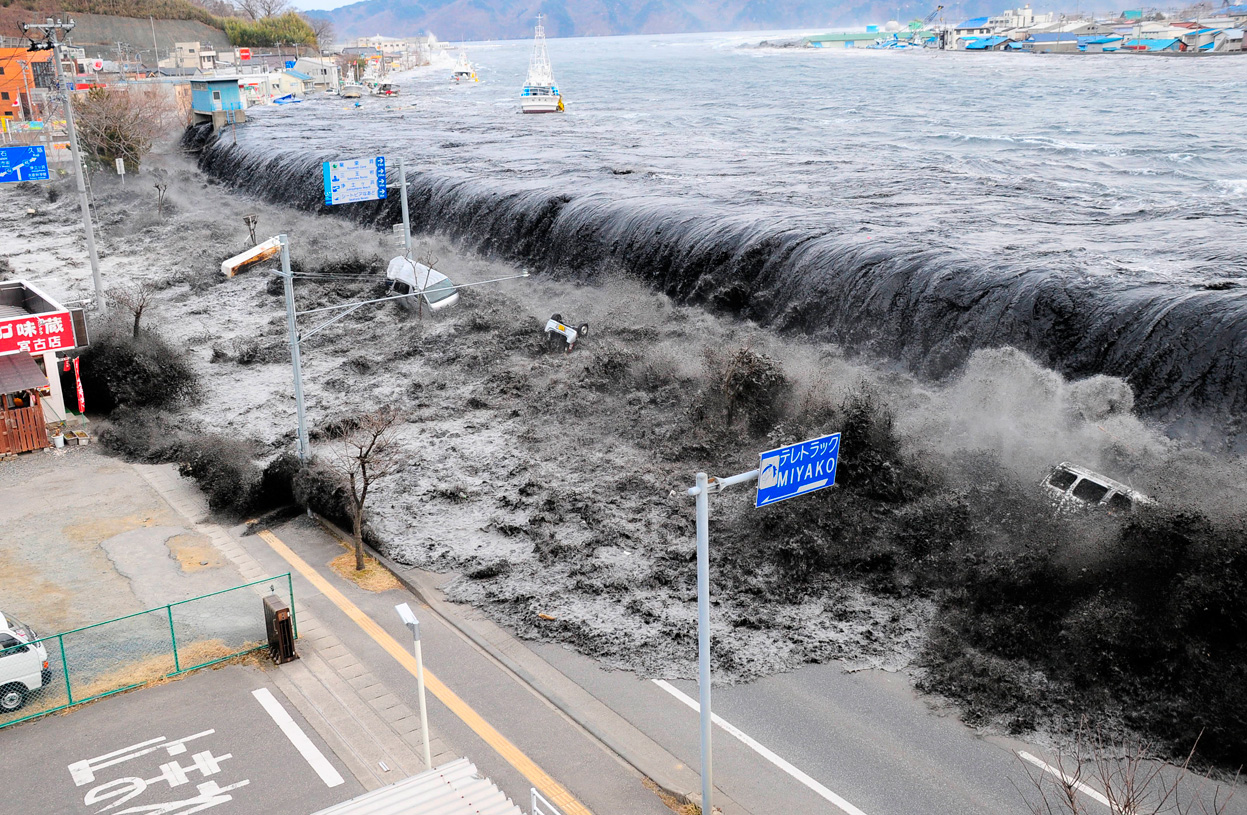
\includegraphics[width=\textwidth]{figures/tsunami-hit.jpg}
  \end{subfigure}
  \begin{subfigure}{.5\textwidth}
    \centering
    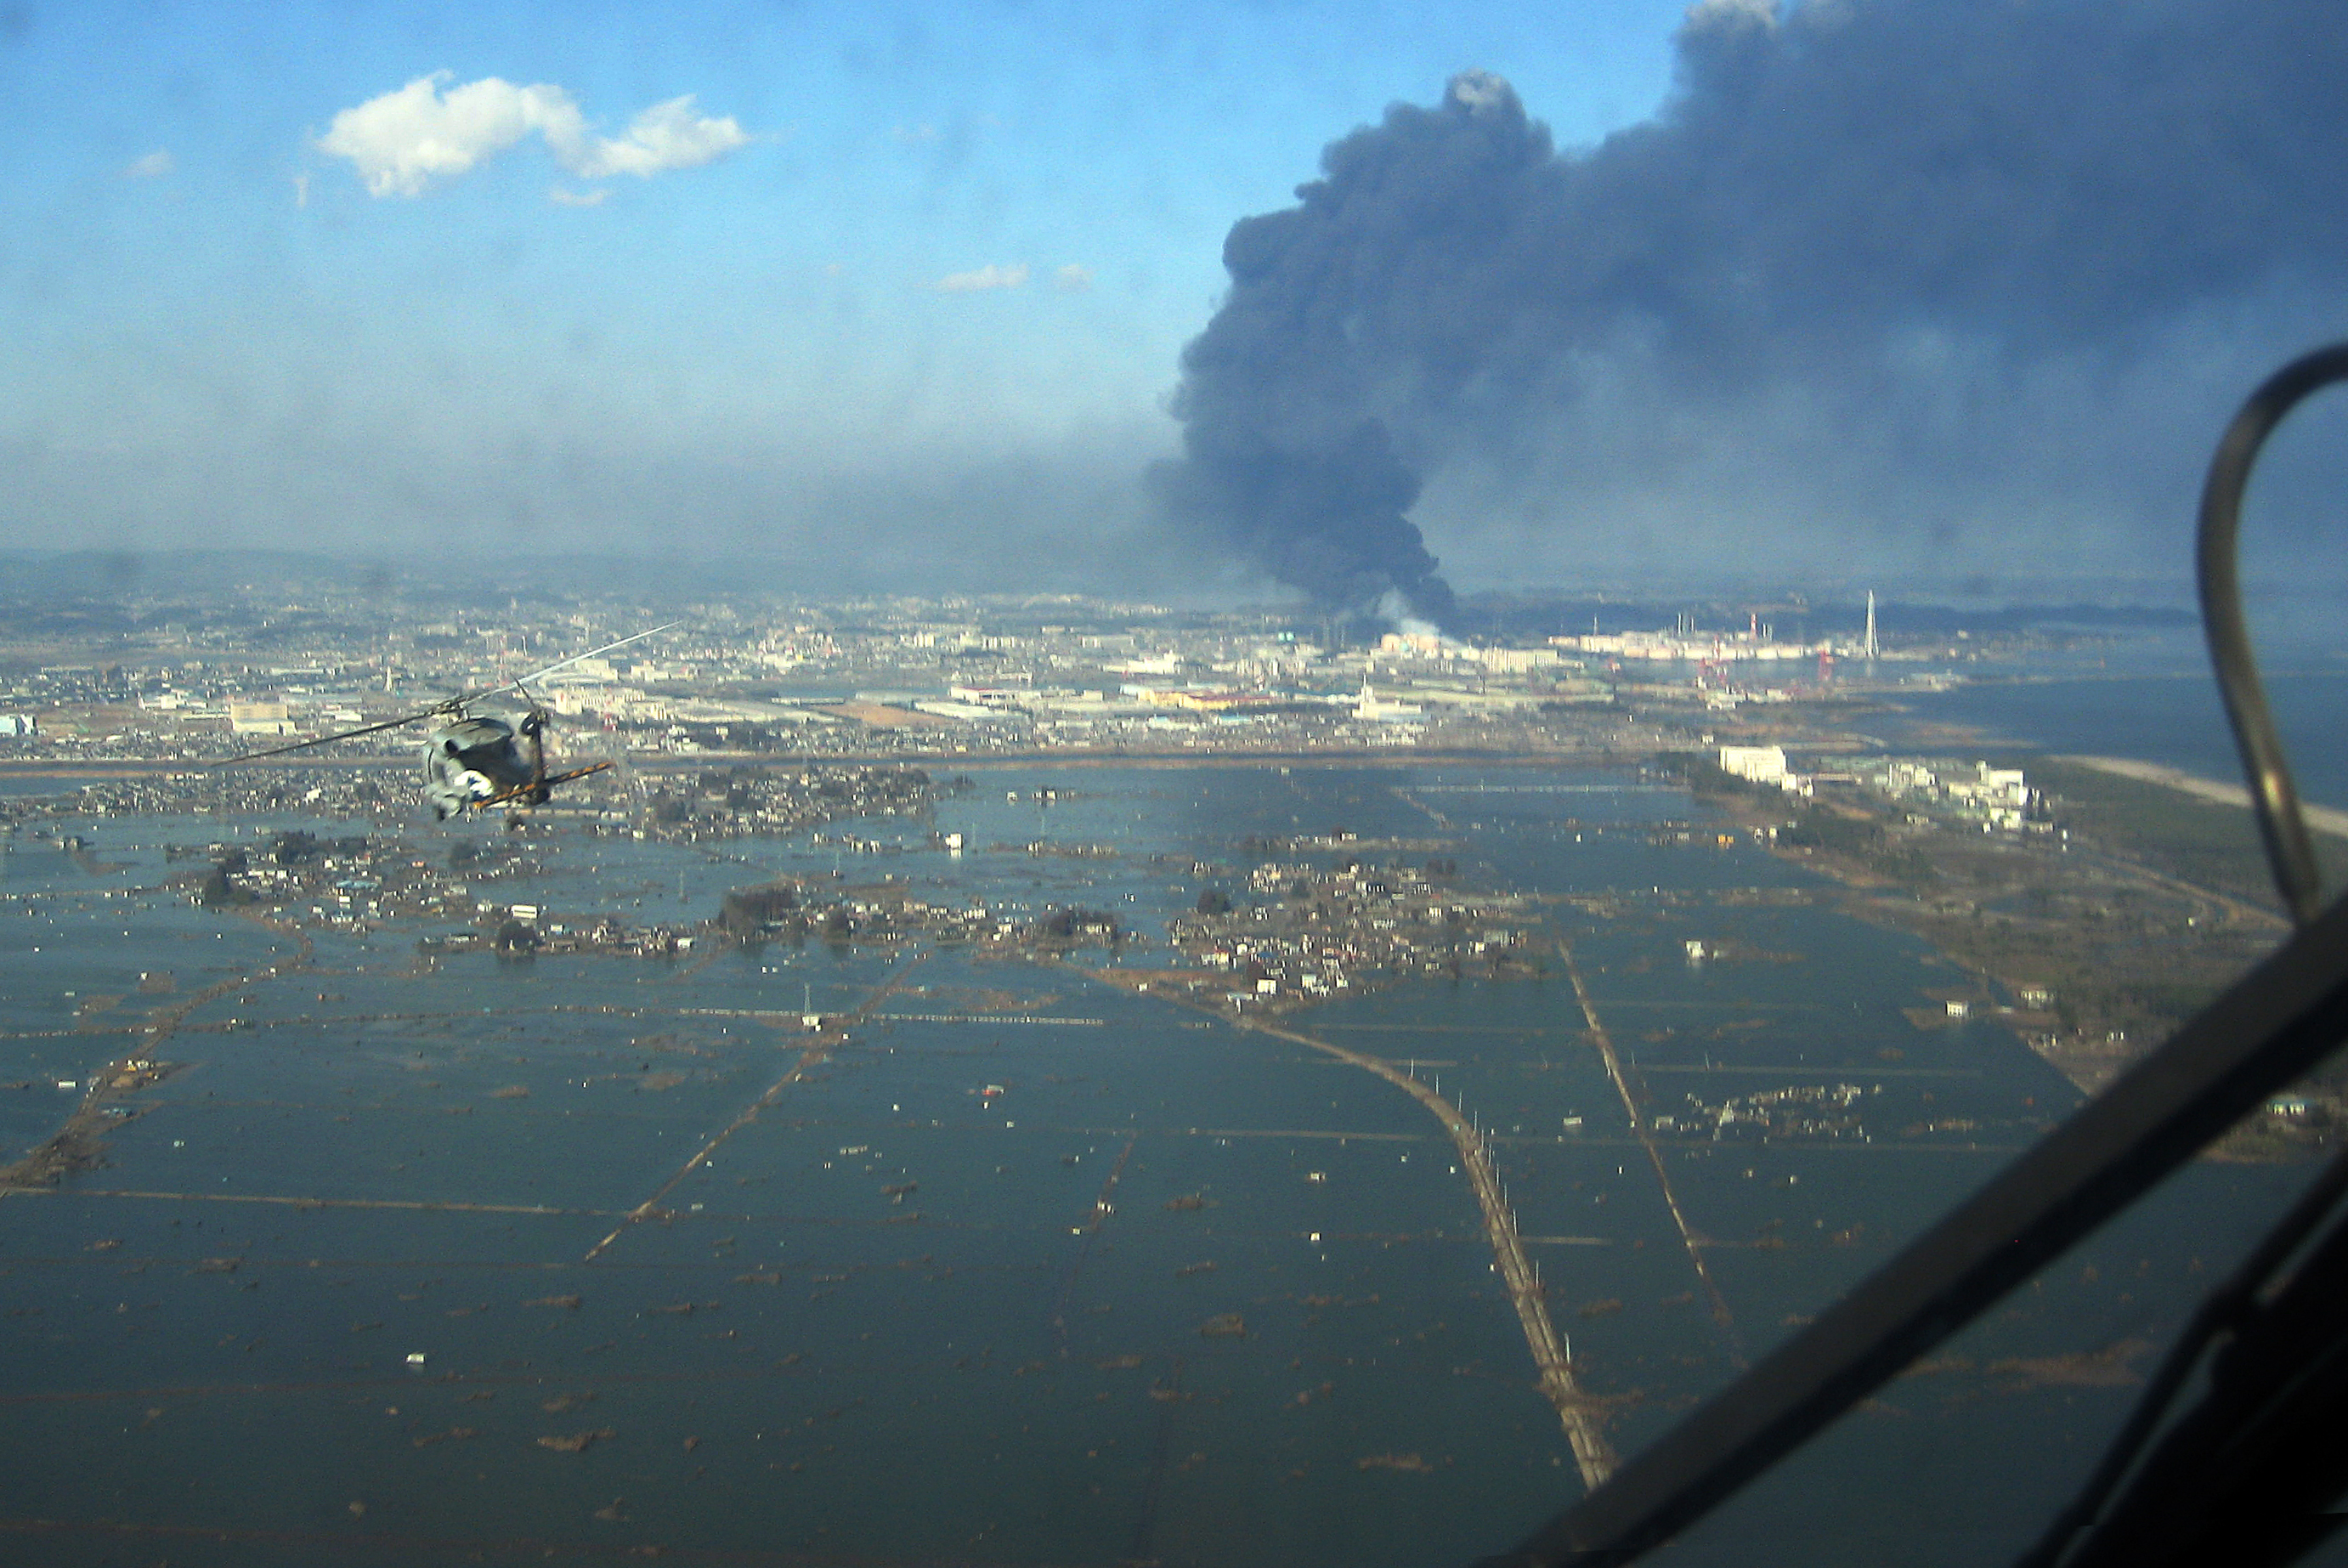
\includegraphics[width=\textwidth]{figures/tsunami-aftermath.jpg}
  \end{subfigure}
  \caption[Πρόσπτωση και καταστροφικά αποτελέσματα τσουνάμι]{Αριστερά πρόσπτωση τσουνάμι
    το 2011 σε παράκτια πόλη της Ιαπωνίας (από \ttt{www.theatlantic.com}) και δεξιά τα
    καταστροφικά αποτελέσματα του ίδιου τσουνάμι στην περιοχή \eng{Sendai}.}
  \label{fig:tsunami-hit-aftermath}
\end{figure}

\paragraph{} Ο όρος τσουνάμι προέρχεται από τα ιαπωνικά και αποτελεί συνδυασμό δύο
ιδεογραμμάτων \eng{kanji} ((τσου)) και ((νάμι)) που σημαίνουν αντίστοιχα ((λιμάνι)) και
((κύμα)), συνολικά δηλαδή ((κύμα στο λιμάνι)). Τα τσουνάμι είναι κύματα που δημιουργούνται
από την απότομη μετατόπιση μεγάλων υδάτινων μαζών, συνήθως ως αποτέλεσμα γεωλογικών
φαινομένων (σεισμοί, εκρήξεις ηφαιστείων, κατολισθήσεις βράχων ή παγετώνων, πτώση
μετεωρίτη) σε παρα/υπο-θαλάσσιες τοποθεσίες (εικόνα \ref{fig:tsunami-generation}). Λόγω
του τρόπου δημιουργίας τους, τα τσουνάμι είναι εντελώς διαφορετικά από τα συνηθισμέντα
κύματα που δημιουργούνται από τον άνεμο, οδεύοντας στον ανοιχτό, βαθύ ωκεανό με τεράστια
ταχύτητα (750 \eng{km/h}) και μήκος κύματος (50-400 \eng{km}), αλλά μικρό ύψος, που
κυμαίνεται από μερικά \eng{cm} έως \eng{1-2 m}. Προσεγγίζοντας πιο ρηχές περιοχές, το κύμα
αλλάζει χαρακτηριστικά, καθώς η ταχύτητα και το μήκος κύματος μειώνονται (κάτω από 80
\eng{km/h} και 20 \eng{km} αντίστοιχα), ενώ το ύψος αυξάνεται. Ωστόσο, μόνο τα πολύ μεγάλα
κύματα παρουσιάζουν ((σπάσιμο)) (\eng{wave breaking}), δηλαδή κατάρρευση της κορυφής τους,
με αποτέλεσμα τα τσουνάμι να μοιάζουν με μεγάλες και απότομες παλίρροιες που προσεγγίζουν
ταχέως την ακτή. Στην εμφάνιση αυτή οφείλεται και η συχνή αλλά εσφαλμένη αναφορά των
κυμάτων αυτών ως παλιρροιακά κύματα, καθώς δεν έχουν καμία σχέση με τις παλίρροιες, οι
οποίες οφείλονται στη βαρυτική έλξη που ασκείται από τον Ήλιο και τη Σελήνη. Λόγω της
τεράστιας ενέργειας που μεταφέρουν (αυτή της μετατόπισης ολόκληρης της υδάτινης στήλης που
προκλήθηκε από το γενεσιουργό συμβάν) τα τσουνάμι είναι καταστροφικά κατά την πρόσπτωσή
τους στις ακτές. Με αυτόν τον τρόπο πήραν και το όνομά τους, καθώς Ιάπωνες ψαράδες που
έβγαιναν στα ανοιχτά δεν αντιλαμβάνονταν το τσουνάμι που περνούσε κάτω από τα πλοία τους,
αντίκριζαν όμως την ολική καταστροφή που είχε προκαλέσει όταν γύριζαν στο λιμάνι. Τα
πρόσφατα τσουνάμι στη νοτιοανατολική Ασία το 2004 και στην Ιαπωνία το 2011 υπήρξαν δύο από
τις μεγαλύτερες φυσικές καταστροφές στη σύγχρονη ιστορία, με τεράστιο αριθμό θυμάτων και
σοβαρές επιπτώσεις, βραχύχρονες (καταστροφή κτιρίων και τοπικών υποδομών) και μακρόχρονες
(καταστροφή και μεγάλη διαρροή ραδιενέργειας στον πυρηνικό αντιδραστήρα \eng{Fukushima
  Daiichi} στην Ιαπωνία).

\begin{figure}[h]
  \begin{subfigure}{.5\textwidth}
    \centering
    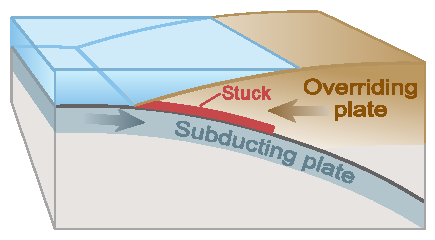
\includegraphics[width=\textwidth]{figures/tsunami-gen-0.pdf}
  \end{subfigure}
  \begin{subfigure}{.5\textwidth}
    \centering
    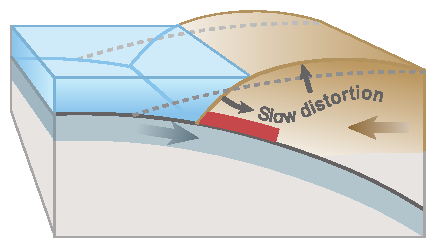
\includegraphics[width=\textwidth]{figures/tsunami-gen-1.pdf}
  \end{subfigure}
  \begin{subfigure}{.5\textwidth}
    \centering
    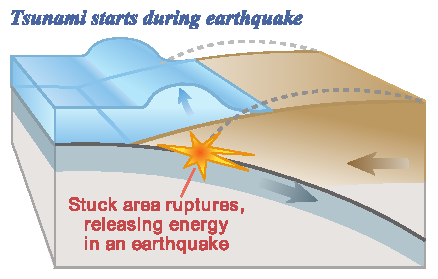
\includegraphics[width=\textwidth]{figures/tsunami-gen-2.pdf}
  \end{subfigure}
  \begin{subfigure}{.5\textwidth}
    \centering
    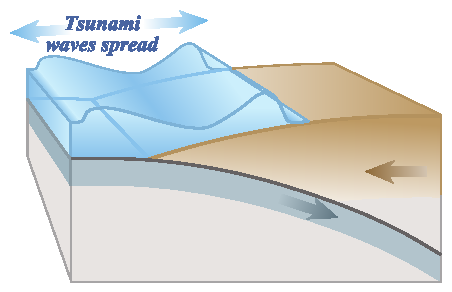
\includegraphics[width=\textwidth]{figures/tsunami-gen-3.pdf}
  \end{subfigure}
  \caption[Γένεση τσουνάμι]{Τα κυριότερα στάδια γένεσης ενός σεισμικού τσουνάμι. Η
    σταδιακή παραμόρφωση που υφίστανται οι αργά κινούμενες γεωλογικές πλάκες εκτονώνεται
    απότομα σε ένα σεισμικό φαινόμενο που μεταφέρει ενέργεια στη υπερκείμενη στήλη νερού,
    η οποία διαδίδεται με το προκύπτον κύμα (από \eng{U.S. Geological Survey, Circular
      1187}).}
  \label{fig:tsunami-generation}
\end{figure}

\paragraph{} Εξαιτίας των σοβαρών τους επιπτώσεων (εικόνα
\ref{fig:tsunami-hit-aftermath}), τα τσουνάμι έχουν αποτελέσει θέμα εκτενούς μελέτης που
αποσκοπεί στην κατανόηση, πρόβλεψη και πρόληψη ζημιών στο μέγιστο δυνατό βαθμό. Η
βιβλιογραφία επικεντρώνεται τόσο την ανάλυση δεδομένων σε παρελθόντα περιστατικά, όσο και
στην μελέτη-προσομοίωση του φαινομένου. Σε μελέτη του 1972 εξετάζονται δύο τσουνάμι της
νεότερης ιστορίας, αυτό της περιοχής \eng{Sanriku} της Ιαπωνίας το 1896 και αυτό στις
Αλεούτιες Νήσους το 1946 \cite{Kanamori1972346}. Το αξιοσημείωτο και με τα δύο αυτά
τσουνάμι είναι οτι παρότι προκλήθηκαν από μικρούς σχετικά σεισμούς υπήρξαν δύο από τα
ισχυρότερα και πιο εκτεταμένα καταγεγραμμένα τσουνάμι της ιστορίας (το δεύτερο από αυτά
οδήγησε στην ίδρυση του \eng{PTWC} τρία χρόνια αργότερα, το 1949). Η δυσαναλογία αυτή
αποτέλεσε και συνεχίζει να αποτελεί αντικείμενο μελέτης, και για το λόγο αυτό έχουν
προταθεί διάφορες κλίμακες μέτρησης της έντασης τέτοιων συμβάντων, με οδηγό ποσότητα την
εκλυόμενη ενέργεια \cite{Kanamori1977} ή μεγέθη του προκύπτοντος τσουνάμι
\cite{ABE19791561}. Η μελέτες των χαρακτηριστικών και επιπτώσεων των τσουνάμι λαμβάνουν
χώρα είτε μακροσκοπικό (δεκάδες χιλιόμετρα) είτε σε επίπεδο ακτογραμμής. Η χρησιμότητα
γραφικής αναπαράστασης -- οπτικοποίησης σε συνδυασμό με μεγάλο όγκο δεδομένων είναι
ιδιαίτερα μεγάλη \cite{Shuto1991171}. Σε πρόσφατη μελέτη σχετικά με το τσουνάμι στον
Ινδικό Ωκεανό το 2004 από προσομοιώσεις σε αριθμητικά μοντέλα σε συνδυασμό με μετρήσεις
του ύψους του νερού και δεδομένα από δορυφόρους προκύπτει οτι το πλάτος, η κατεύθυνση και
διάδοση των κυμάτων καθορίστηκαν κυρίως από τον προσανατολισμό και ένταση της σεισμικής
πηγής κατά μήκος του ρήγματος και ακολούθως από το φαινόμενο κυματοδήγησης από
μεσοωκεάνιες κορυφογραμμές \cite{Titov23092005}. Σε άλλη μελέτη του ίδιου γεγονότος, έγινε
μεγάλης κλίμακας προσομοίωση, αφότου προσδιορίστηκε κατά το δυνατόν ακριβέστερα η σεισμική
δόνηση που προκάλεσε το τσουνάμι \cite{Grilli2007414}. Βάσει διαφόρων δεδομένων από
σεισμογράφους, μετρητές παλίρροιας, σταθμούς \eng{GPS}, δορυφόρους, παρατηρήσεις και
καταγραφές αυτόπτων μαρτύρων, μετρήσεις στις πληγείσες ακτογραμμές και χαρτογράφηση των
αλλαγών στον πυθμένα κοντά στο επίκεντρο του σεισμού, σε συνδυασμό με γεωλογικές και
σεισμολογικές παραμέτρους, δημιουργήθηκε μια εικονική σεισμική πηγή. Η πηγή αυτή
χρησιμοποιήθηκε για να κατασκευαστεί ένα αριθμητικό μοντέλο για τη γένεση, διάδοση και
πρόσπτωση στις ακτογραμμές του τσουνάμι, λαμβάνοντας υπόψη συχνοτική διασπορά και μη
γραμμικότητα. Τα αποτελέσματα της προσομοίωσης συμφωνούν τόσο σε μεγέθη όσο και χρονικά με
μετρήσεις του πραγματικού φαινομένου, γεγονός που την καθιστά πρόσφορη σαν βάση για
μεγαλύτερης λεπτομέρειας μελέτες, ενώ παράλληλα καταδεικνύει τη χρησιμότητα των
προσομοιώσεων για την κατανόηση των μηχανισμών γένεσης και εκδήλωσης των τσουνάμι.

\subsection{Συνεισφορά}
\paragraph{} Σκοπός της παρούσας εργασίας ήταν η ανάπτυξη εφαρμογής για την προσομοίωση
της πρόσπτωσης ενός τσουνάμι σε τοπικό επίπεδο ακτογραμμής. Σε αυτήν την κλίμακα, το
ενδιαφέρον εστιάζεται πρωτίστως στη ζημιά που θα προκληθεί από το κύμα κατά την εισβολή
του στη στεριά. Ο καθοριστικός παράγοντας για την πρόβλεψη της ζημιάς στην ακτογραμμή
είναι η κατανομή της μεταδιδόμενης ορμής του κύματος στα τμήματα της ακτογραμμής με τα
οποία έρχεται σε επαφή, τόσο στο χώρο όσο και στο χρόνο. Αυτό σημαίνει οτι θα πρέπει κατά
τη διάρκεια της προσομοίωσης να υπολογίζεται το ποσό ορμής που δέχθηκε κάθε τμήμα της
ακτογραμμής, όπως και ο χρόνος και ο ρυθμός με τον οποίο έγινε αυτό. Για το σκοπό αυτό
κατά την επιλογή του μοντέλου ρευστού, της μεθόδου προσομοίωσης αλλά και την ανάπτυξη του
προγράμματος δίνεται ιδιαίτερη έμφαση στη διατήρηση της ορμή και καταγραφή της μετάδοσής
της στην ακτογραμμή, κάτι το οποίο δεν έχει γίνει σε εκτεταμένο βαθμό σε υπάρχουσες
προσομοιώσεις του φαινομένου \cite{debroux2001three}.

\paragraph{} Ο κυριότερος λόγος πίσω από την έλλειψη αυτή είναι τα καταστροφικά
αποτελέσματα που έχουν όλα τα τσουνάμι στις περιοχές που πλήττουν, χωρίς παράλληλα να
είναι προς το παρόν εφικτά μέτρα ουσιαστικής αποτροπής των συνεπειών τους, πλην των
ενισχυμένων κυματοθραυστών που βρίσκονται εγκατεστημένοι για την προστασία περιοχών υψηλού
κινδύνου. Ωστόσο η ποσοτική πληροφορία που παρέχουν εφαρμογές σαν αυτή που αναπτύχθηκε στα
πλαίσια αυτής της εργασίας μπορούν να χρησιμοποιηθούν σε πλείστους τομέις, όπως η
πολεοδομία και ο σχεδιασμός παράκτιων εγκαταστάσεων (εργοστάσια, γέφυρες, φράγματα, κλπ)
με στόχο την αύξηση της ασφάλειας σε περίπτωση τσουνάμι. Αν και το τσουνάμι είναι ένα
υπερβολικά μεγάλο για τα ανθρώπινα δεδομένα φαινόμενο, η ποσοτική μελέτη των επιπτώσεών
του μπορεί να συνδράμει σημαντικά στην προστασία από αυτές, όπως ακριβώς έχει συμβεί με
τους σεισμούς στην πορεία της ιστορίας (ένα σχετικό φαινόμενο ίδιας έκτασης και εξίσου
καταστροφικό).

\paragraph{} Στην εφαρμογή που αναπτύχθηκε, η προσομοίωση λαμβάνει ως παραμέτρους το
τρισδιάστατο μοντέλο της ακτογραμμής, τις αρχικές συνθήκες του ρευστού, το χρονικό βήμα
μεταξύ των εξαγόμενων στιγμιοτύπων της προσομοίωσης καθώς και την επιθυμητή ανάλυση για τη
διακριτοποίηση του ρευστού σε σωματίδια. Τα αρχεία εξόδου περιέχουν πληροφορίες σχετικά με
το ρευστό (θέση, δυνάμεις πίεσης -- ιξώδους, κλπ), τις δυνάμεις που ασκήθηκαν ακτογραμμή,
αλλά και αθροιστικές πληροφορίες με τη μορφή βαθμωτών πεδίων στο χώρο. Τα δεδομένα αυτά
μπορούν να οπτικοποιηθούν με πολλούς τρόπους με τη βοήθεια ειδικών προγραμμάτων, με στόχο
την εύκολη οπτική αντίληψη και επεξεργασία της πληροφορίας. Η δυνατότητα ευέλικτης
οπτικοποίησης είναι ιδιαίτερα σημαντική, καθώς τα δεδομένα εξόδου μπορούν να ιδωθούν
ταυτόχρονα ανά συνδυασμούς ή να χρησιμοποιηθούν σαν πηγές για οπτικοποιήσεις συσχέτισης
μεταξύ τους.

\subsection{Δομή της εργασίας}

\paragraph{} Η εργασία αποτελείται από τέσσερα κεφάλαια πέραν της εισαγωγής, σκοπός των
οποίων είναι να αναλύσουν το πρόβλημα, τις ήδη υπάρχουσες λύσεις, την ανάπτυξη της
πα\-ρού\-σας εφαρμογής, τα αποτελέσματα που παρήχθησαν από αυτή καθώς και μια κριτική σε
συνδυασμό με προτάσεις για μελλοντικές επέκτασεις της.

\paragraph{} Στο δεύτερο κεφάλαιο γίνεται μια σύντομη αλλά αναλυτική έκθεση και σύγκριση
των διαφόρων μεθόδων προσομοίωσης ρευστών που υπήρξαν υποψήφιες για τη συγκεκριμένη
εφαρμογή. Πρώτη οικογένεια μεθόδων είναι αυτές των πεπερασμένων στοιχείων, οι οποίες
βασίζονται στην αριθμητική επίλυση των εξισώσεων \eng{Navier-Stokes} μετά την κατάλληλη
διακριτοποίηση του χώρου της προσομοίωσης. Σε αντίθεση με αυτές, οι δύο άλλες μέθοδοι που
εξετάζονται είναι σωματιδιακές μέθοδοι, που όπως εξηγείται ταιριάζουν καλύτερα στη φύση
του προβλήματος. Η πρώτη από αυτές τις μεθόδους είναι η \eng{Lattice Boltzmann}, κατά την
οποία ο χώρος της προσομοίωσης διακριτοποιείται σε πλέγμα και το ρευστό προσομοιώνεται
βάσει της μεσοσκοπικής θεώρησής του, σύμφωνα με την κινητική θεωρία. Η άλλη μέθοδος, η
οποία είναι και αυτή που υιοθετείται τελικά είναι η \eng{Smoothed Particle Hydrodynamics},
κατά την οποία δεν διακριτοποιείται ο χώρος της προσομοίωσης, αλλά το ίδιο το ρευστό σε
σωματίδια. Τα σωματίδια φέρουν ιδιότητες του ρευστού και χρησιμοποιούνται σαν σημεία
δειγματοληψίας και παρεμβολής για τον υπολογισμό των ιδιοτήτων αυτών στο χώρο. Στη
συνέχεια παρουσιάζεται μια συγκριτική σύνοψη όπου αναλύονται τα επιμέρους μειονεκτήματα
και πλεονεκτήματα της κάθε μεθόδου.

\paragraph{} Το τρίτο κεφάλαιο αποτελεί τη λεπτομερή τεκμηρίωση της εφαρμογής που
αναπτύχθηκε. Το κεφάλαιο αυτό ξεκινά με μια επισκόπηση της \eng{Bullet}, της μηχανής
φυσικής που χρησιμοποιήθηκε για την ενσωμάτωση απαραίτητων μηχανικών αλληλεπιδράσεων στο
μοντέλο της προσομοίωσης, αλλά και λόγω της υποδομής που προσφέρει για το χειρισμό και
καταγραφή αυτών. Κατά τη διάρκεια της προσομοίωσης, η μηχανή φυσικής συνεργάζεται με την
μηχανή \eng{SPH} που αναπτύχθηκε καθώς διαδέχεται η μία την άλλη κατά τον υπολογισμό της
δυναμικής συμπεριφοράς του ρευστού. Στη συνέχεια εξηγείται αναλυτικά η αναπαράσταση της
ακτογραμμής και του ρευστού με αντικείμενα που δημιουργούνται στον εικονικό κόσμο της
\eng{Bullet}. Κατόπιν αναφέρεται η διαδικασία με την οποία συντελείται η αρχικοποίηση του
ρευστού και καθορίζεται το χρονικό βήμα της προσομοίωσης σε συνδυασμό με άλλες παραμέτρους
που σχετίζονται τόσο με τη διακριτοποίηση όσο και με τις αρχικές συνθήκες. Στο τμήμα αυτό
εκτίθενται και οι λεπτομέρειες σχεδιασμού και υλοποίησης του \eng{LP grid}, μιας ειδικής
δομής δεδομένων που αναπτύχθηκε με βάση τα μοτίβα πρόσβασης στα σωματίδια του ρευστού κατά
την εκτέλεση της μεθόδου \eng{SPH}. Απώτερος σκοπός της εν λόγω δομής ήταν η
βελτιστοποίηση της ταχύτητας ανάκτησης των σωματιδίων και διάταξης αποθήκευσης από και
προς τη μνήμη, ενώ επιπρόσθετα παρέχονται ρουτίνες αρχικοποίησης και ενημέρωσής της σε
μορφή ψευδοκώδικα. Τέλος, παρατίθεται μια σύνοψη της υλοποίησης του αλγορίθμου
προσομοίωσης, όπου ενσωματώνονται όλες οι προαναφερθείσες διαδικασίες, σε συνδυασμό με την
εξαγωγή των δεδομένων.

\paragraph{} Στο τέταρτο και πέμπτο κεφάλαιο γίνεται μια παρουσίαση και σχολιασμός
αποτελεσμάτων που παρήχθησαν από το πρόγραμμα προσομοίωσης και μία κριτική σε συνδυασμό με
προτάσεις για μελλοντική επέκτασή του αντίστοιχα. Τα αποτελέσματα αφορούν προσομοιώσεις
που έγιναν σε διαφορετικά μοντέλα ακτογραμμής και περιλαμβάνουν οπτικοποιήσεις διαφόρων
μεγεθών και στοιχείων (όπως δυνάμεις εντός του ρευστού και ανακατασκευασμένη επιφάνεια,
οπτικοποίηση ώσεων από το ρευστό στην ακτογραμμή διακριτά και σε αθροιστικό
\eng{heatmap}). Τέλος, αναφέρονται τα κυριότερα αδύναμα σημεία της εφαρμογής όπως
προκύπτουν από την εμπειρία κατά την ανάπτυξη και χρήση της αλλά και από δεδομένα
προερχόμενα από τα αποτελέσματα και μετρήσεις απόδοσης, ενώ προτείνονται πιθανοί τρόποι
αντιμετώπισής τους σαν μελλοντικές επεκτάσεις της εργασίας.

%%% Local Variables:
%%% mode: latex
%%% TeX-master: "report"
%%% End:
